
\documentclass{article}
\usepackage[utf8]{inputenc}
\usepackage{ctex}
\usepackage{tikz}
\usetikzlibrary{shapes.geometric, arrows.meta, positioning, calc}
\usepackage{amsmath}
\usepackage{geometry}
\geometry{a4paper, margin=1in}

\tikzset{
    entity/.style={rectangle, draw, thick, minimum width=2cm, minimum height=1cm, align=center},
    weak entity/.style={rectangle, draw, thick, double, minimum width=2cm, minimum height=1cm, align=center},
    relationship/.style={diamond, draw, thick, aspect=2, minimum width=2.5cm, minimum height=1cm, align=center},
    weak relationship/.style={diamond, draw, thick, double, aspect=2, minimum width=2.5cm, minimum height=1cm, align=center},
    attribute/.style={ellipse, draw, minimum width=1.5cm, minimum height=0.8cm, align=center},
    multi attribute/.style={ellipse, draw, double, minimum width=1.5cm, minimum height=0.8cm, align=center},
    isa/.style={regular polygon, regular polygon sides=3, draw, thick, shape border rotate=180, inner sep=0pt, minimum size=1cm}
}

\begin{document}

\section*{Exercise 6.1}
\textbf{问题}：为车辆保险公司构建一张E-R图，其每位客户拥有一辆或多辆车。每辆车关联零次或任意多次事故的记录。每张保险单为一辆或多辆车投保，并与一次或多次保费支付相关联。每次支付只针对一段特定的时间，具有关联的到期日和缴费日。

\vspace{0.5cm}
\textbf{解答}：
\begin{center}
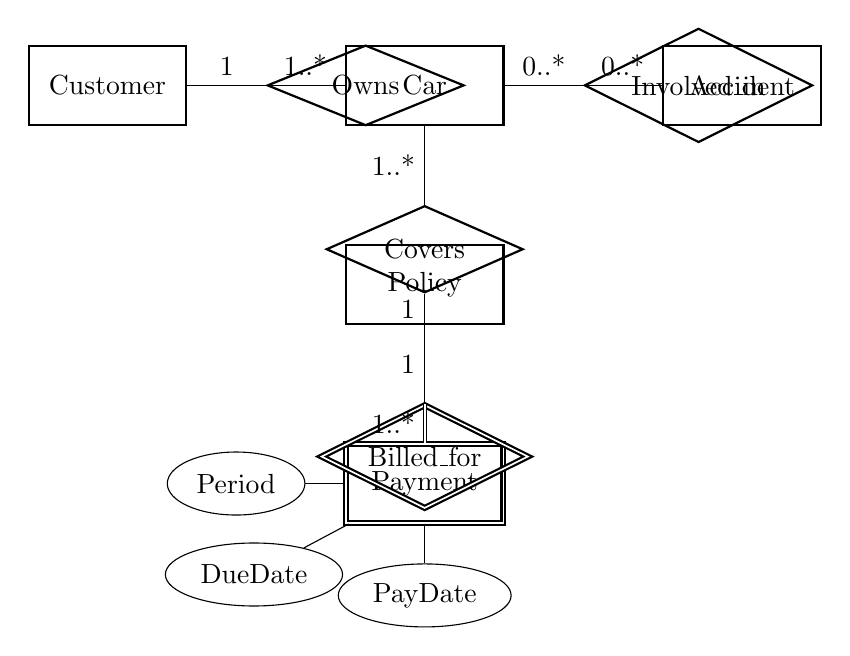
\begin{tikzpicture}[node distance=1.5cm and 2cm]
    % Entities
    \node[entity] (customer) {Customer};
    \node[entity, right=of customer] (car) {Car};
    \node[entity, right=of car] (accident) {Accident};
    \node[entity, below=of car] (policy) {Policy};
    \node[weak entity, below=of policy] (payment) {Payment};

    % Relationships
    \node[relationship, right=1cm of customer] (owns) {Owns};
    \node[relationship, right=1cm of car] (involved) {Involved\_in};
    \node[relationship, below=1cm of car] (covers) {Covers};
    \node[weak relationship, below=1cm of policy] (billed) {Billed\_for};

    % Links
    \draw (customer) -- node[above] {1} (owns);
    \draw (owns) -- node[above] {1..*} (car);
    
    \draw (car) -- node[above] {0..*} (involved);
    \draw (involved) -- node[above] {0..*} (accident);
    
    \draw (policy) -- node[left] {1} (covers);
    \draw (covers) -- node[left] {1..*} (car);
    
    \draw (policy) -- node[left] {1} (billed);
    \draw[double] (billed) -- node[left] {1..*} (payment);

    % Attributes for Payment (Weak Entity)
    \node[attribute, left=0.5cm of payment] (p_period) {Period};
    \node[attribute, below left=0.5cm of payment] (p_due) {DueDate};
    \node[attribute, below=0.5cm of payment] (p_pay) {PayDate};
    \draw (payment) -- (p_period);
    \draw (payment) -- (p_due);
    \draw (payment) -- (p_pay);
\end{tikzpicture}
\end{center}

\vspace{1cm}
%------------------------------------------------

\section*{Exercise 6.2}
\textbf{问题}：考虑一个数据库，它包含来自大学模式的 student、course 和 section 实体集，并且另外还记录了学生在不同课程段的不同考试中所获得的分数。
\begin{itemize}
    \item a. 构建一张 E-R 图，将考试建模为实体，并使用三元联系作为设计的一部分。
    \item b. 构造一张可替代的 E-R 图，它只使用 student 和 section 之间的二元联系。保证在特定的 student 和 section 对之间只存在一个联系，而且可以表示出学生在不同考试中所得的分数。
\end{itemize}

\vspace{0.5cm}
\textbf{解答 a (三元联系)}：
\begin{center}
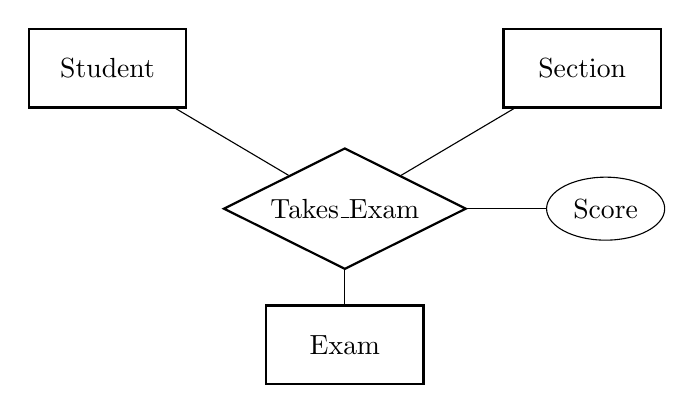
\begin{tikzpicture}[node distance=2cm]
    \node[entity] (student) {Student};
    \node[entity, right=4cm of student] (section) {Section};
    \node[entity, below=3cm of $(student)!0.5!(section)$] (exam) {Exam};
    \node[relationship, below=1cm of $(student)!0.5!(section)$] (takes) {Takes\_Exam};
    \node[attribute, right=1cm of takes] (score) {Score};

    \draw (student) -- (takes);
    \draw (section) -- (takes);
    \draw (exam) -- (takes);
    \draw (takes) -- (score);
\end{tikzpicture}
\end{center}

\vspace{0.5cm}
\textbf{解答 b (二元联系 + 复合多值属性)}：
\begin{center}
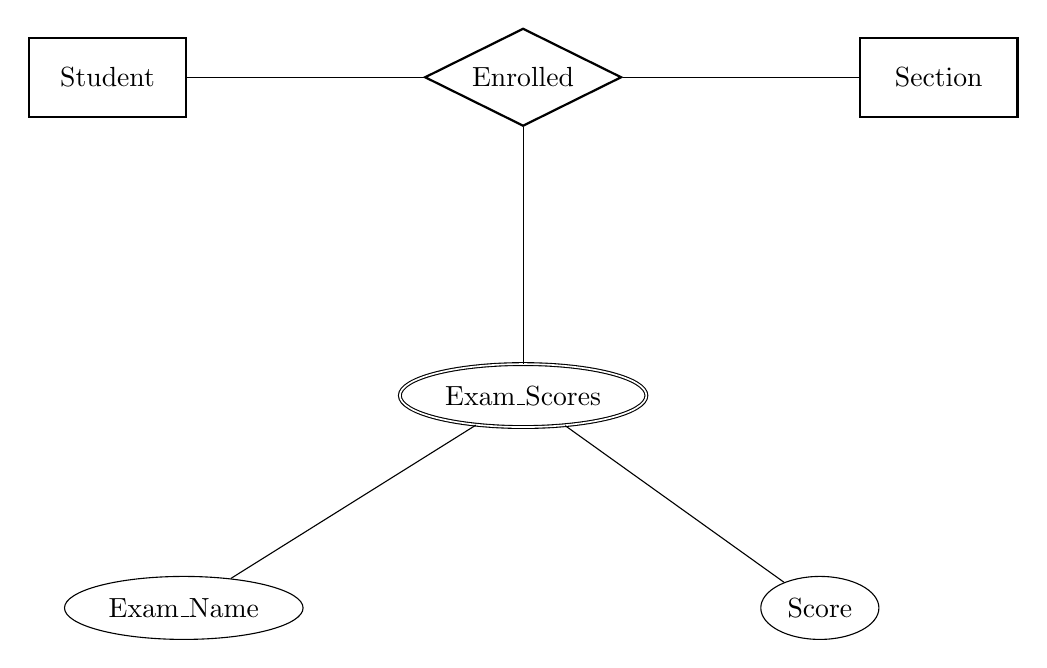
\begin{tikzpicture}[node distance=3cm]
    \node[entity] (student) {Student};
    \node[relationship, right=of student] (enrolled) {Enrolled};
    \node[entity, right=of enrolled] (section) {Section};
    
    \node[multi attribute, below=of enrolled] (examscores) {Exam\_Scores};
    \node[attribute, below left=of examscores] (examname) {Exam\_Name};
    \node[attribute, below right=of examscores] (score) {Score};

    \draw (student) -- (enrolled);
    \draw (section) -- (enrolled);
    \draw (enrolled) -- (examscores);
    \draw (examscores) -- (examname);
    \draw (examscores) -- (score);
\end{tikzpicture}
\end{center}

\vspace{1cm}
%------------------------------------------------

\section*{Exercise 6.21}
\textbf{问题}：考虑图 6-30 中对在线书店建模的 E-R 图。
\begin{itemize}
    \item a. 假设书店增加了蓝光光盘和可下载视频。相同的商品可能以一种或两种格式存在，不同格式价格不同。绘制部分 E-R 图，仅显示视频相关部分。
    \item b. 扩展完整的 E-R 图，从而对包含书、蓝光或下载视频的任意组合的购物篮进行建模。
\end{itemize}

\vspace{0.5cm}
\textbf{解答 a}：由于同一视频可以有不同的格式（蓝光、下载）且价格不同，使用弱实体集 \texttt{Video\_Format} 来表示。
\begin{center}
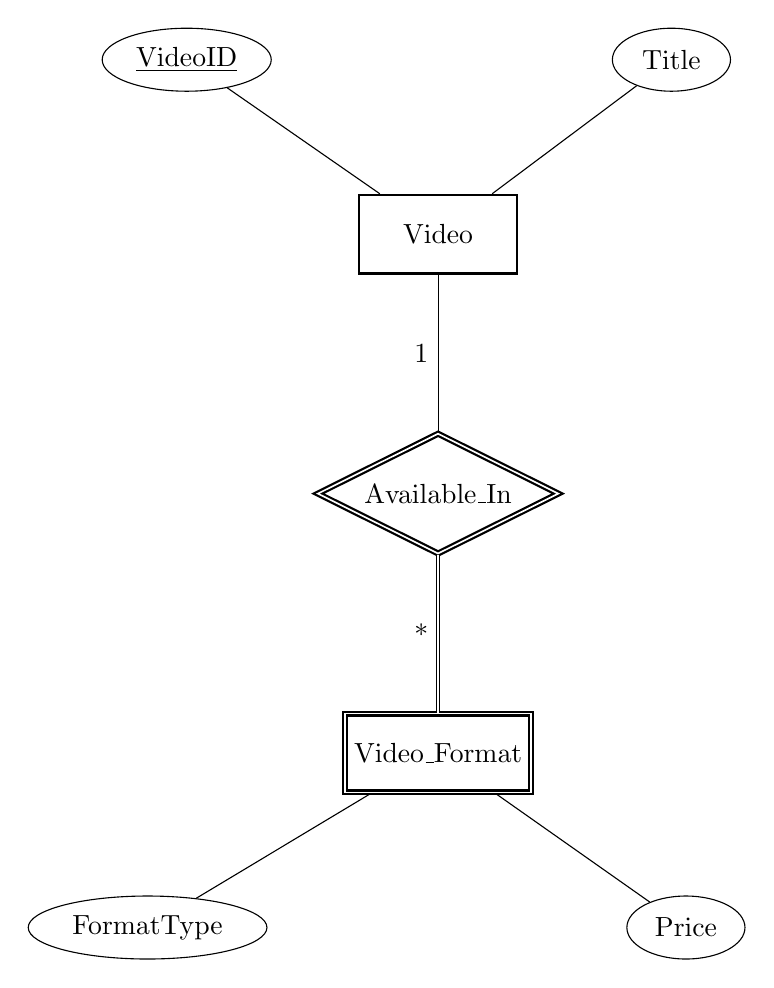
\begin{tikzpicture}[node distance=2cm]
    \node[entity] (video) {Video};
    \node[attribute, above left=of video] (v_id) {\underline{VideoID}};
    \node[attribute, above right=of video] (v_title) {Title};
    
    \node[weak relationship, below=of video] (available_in) {Available\_In};
    
    \node[weak entity, below=of available_in] (format) {Video\_Format};
    \node[attribute, below left=of format] (f_type) {\dasheduline{FormatType}};
    \node[attribute, below right=of format] (f_price) {Price};

    \draw (video) -- (v_id);
    \draw (video) -- (v_title);
    \draw (video) -- node[left] {1} (available_in);
    \draw[double] (available_in) -- node[left] {*} (format);
    \draw (format) -- (f_type);
    \draw (format) -- (f_price);
\end{tikzpicture}
\end{center}

\vspace{0.5cm}
\textbf{解答 b}：引入一个通用的超类 \texttt{Purchasable\_Item}，让 \texttt{Book} 和 \texttt{Video\_Format} 继承自它，\texttt{Shopping\_Basket} 包含该超类。
\begin{center}
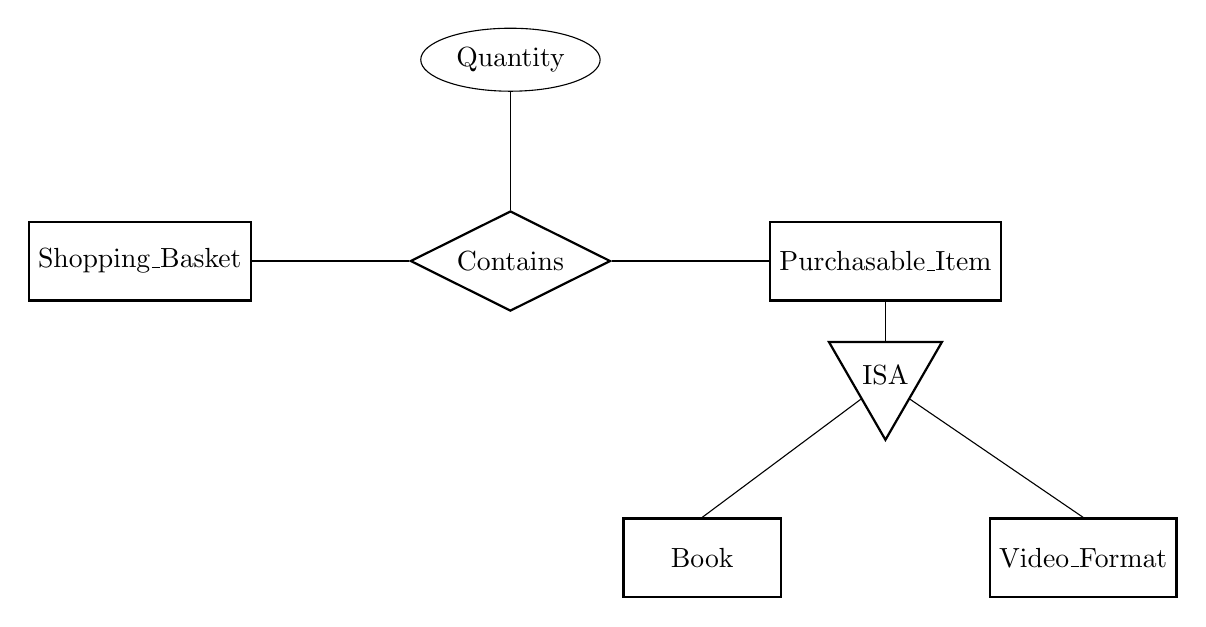
\begin{tikzpicture}[node distance=1.5cm]
    \node[entity] (item) {Purchasable\_Item};
    \node[isa, below=0.5cm of item] (isa) {ISA};
    
    \node[entity, below left=1.5cm and 1cm of isa] (book) {Book};
    \node[entity, below right=1.5cm and 1cm of isa] (vformat) {Video\_Format};
    
    \node[relationship, left=2cm of item] (contains) {Contains};
    \node[entity, left=2cm of contains] (basket) {Shopping\_Basket};
    \node[attribute, above=of contains] (qty) {Quantity};

    \draw (item) -- (isa.north);
    \draw (isa.south west) -- (book.north);
    \draw (isa.south east) -- (vformat.north);
    
    \draw (basket) -- (contains);
    \draw (contains) -- (item);
    \draw (contains) -- (qty);
\end{tikzpicture}
\end{center}

\vspace{1cm}
%------------------------------------------------

\section*{Exercise 6.22}
\textbf{问题}：为汽车公司设计数据库以维护客户、经销商库存和销售订购。车辆由 VIN 标识，是特定品牌和模型。模型有可用选项，特定车辆包含其中部分选项。

\vspace{0.5cm}
\textbf{解答 (关系模式与约束)}：
\begin{itemize}
    \item \textbf{Brand}(\underline{BrandName})
    \item \textbf{Model}(\underline{ModelID}, ModelName, BrandName) \\
    \textit{外码}: BrandName 引用 Brand.BrandName
    \item \textbf{Option}(\underline{OptionCode}, Description)
    \item \textbf{Model\_Options}(\underline{ModelID, OptionCode}) \\
    \textit{外码}: ModelID 引用 Model.ModelID, OptionCode 引用 Option.OptionCode
    \item \textbf{Dealer}(\underline{DealerID}, Name, Location)
    \item \textbf{Salesperson}(\underline{EmpID}, Name, DealerID) \\
    \textit{外码}: DealerID 引用 Dealer.DealerID
    \item \textbf{Customer}(\underline{CustID}, Name, Phone)
    \item \textbf{Car}(\underline{VIN}, ModelID, DealerID) \\
    \textit{外码}: ModelID 引用 Model.ModelID, DealerID 引用 Dealer.DealerID
    \item \textbf{Car\_Options}(\underline{VIN, OptionCode}) \\
    \textit{外码}: VIN 引用 Car.VIN, OptionCode 引用 Option.OptionCode
    \item \textbf{Sales\_Order}(\underline{VIN}, CustID, EmpID, OrderDate, Price) \\
    \textit{主码}: VIN (因为一辆实体车只能被售出一次) \\
    \textit{外码}: VIN 引用 Car.VIN, CustID 引用 Customer.CustID, EmpID 引用 Salesperson.EmpID
\end{itemize}

\vspace{1cm}
%------------------------------------------------

\section*{Exercise 6.24}
\textbf{问题}：为航空公司设计数据库。追踪客户、预订、航班及状态、座位分配、时刻表和路线。

\vspace{0.5cm}
\textbf{解答 (关系模式与约束)}：
\begin{itemize}
    \item \textbf{Customer}(\underline{CustID}, Name, Phone, Email)
    \item \textbf{Reservation}(\underline{ResNo}, CustID, ResDate) \\
    \textit{外码}: CustID 引用 Customer.CustID
    \item \textbf{Flight\_Route}(\underline{RouteID}, Source, Destination) 
    \item \textbf{Flight\_Schedule}(\underline{FlightNo}, RouteID, DepartureTime, ArrivalTime) \\
    \textit{外码}: RouteID 引用 Flight\_Route.RouteID
    \item \textbf{Flight\_Instance}(\underline{FlightNo, FlightDate}, Status) \\
    \textit{外码}: FlightNo 引用 Flight\_Schedule.FlightNo
    \item \textbf{Seat\_Assignment}(\underline{FlightNo, FlightDate, SeatNo}, Class, ResNo) \\
    \textit{外码}: (FlightNo, FlightDate) 引用 Flight\_Instance, ResNo 引用 Reservation.ResNo
\end{itemize}

\end{document}
